\documentclass[11pt]{article}
\usepackage[utf8]{inputenc}
\usepackage[T1]{fontenc}
\usepackage[spanish]{babel}
\usepackage[margin=2.5cm]{geometry}
\usepackage{graphicx}
\usepackage{hyperref}
\usepackage{fancyhdr}

\hypersetup{colorlinks=true, linkcolor=black, urlcolor=blue, citecolor=black}
\pagestyle{fancy}
\fancyhf{}
\fancyhead[L]{Gobierno del dato y toma de decisiones -- Actividad 1}
\fancyhead[R]{\thepage}
\renewcommand{\headrulewidth}{0.4pt}

\title{\textbf{Actividad 1. Laboratorio (individual):\\ Almacenes de datos, catálogo y ETL}}
\date{\today}

\begin{document}

\begin{titlepage}
    \centering
    \vspace*{2cm}
    {\Large Gobierno del dato y toma de decisiones\par}
    \vspace{2cm}
    {\Huge\bfseries Actividad 1. Laboratorio (individual):\par}
    {\Huge\bfseries Almacenes de datos, catálogo y ETL\par}
    \vspace{3cm}
    {\large Nombre y Apellidos: David Vicente Moya \par}
    \vspace{0.5cm}
    {\large \today \par}
    \vfill
\end{titlepage}

\tableofcontents
\newpage

\section{Parte I. Estrategia y carga de datos}

\subsection{C) Espacios de trabajo}

Se han creado tres espacios de trabajo en Dremio: \textbf{Analista 1}, \textbf{Analista 2}
y \textbf{Analista 3}.

\subsubsection{Limitación de Dremio OSS: wiki de espacios de trabajo}

El enunciado pide documentar cada espacio de trabajo con una wiki descriptiva, de forma
análoga a la wiki de cada dataset. Sin embargo, en la versión de Dremio Community (OSS)
utilizada en esta práctica, el panel de \emph{Wiki} solo ofrece edición de contenido para
\textbf{datasets}, no para \textbf{espacios}. Como se observa en la
Figura~\ref{fig:wiki-espacio}, al abrir un espacio (Analista~1) el panel derecho muestra la
sección \emph{Wiki} con el mensaje \texttt{"No wiki content yet"}, pero no expone ningún
control de edición: ni botón, ni icono, ni área de texto interactiva al pasar el cursor o
al hacer clic sobre ella. Esta limitación es consistente en los tres espacios creados.

\begin{figure}[h]
    \centering
    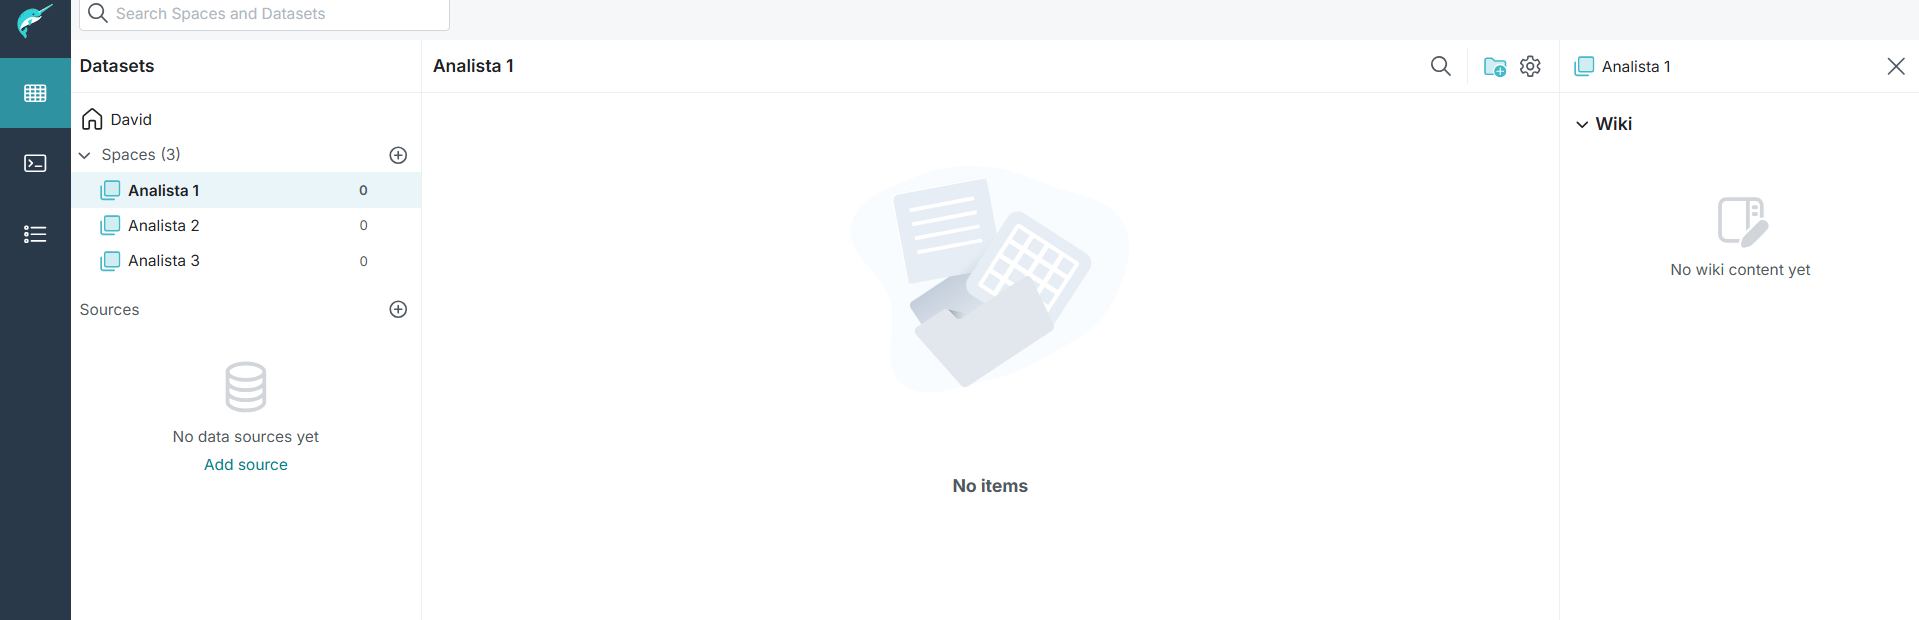
\includegraphics[width=0.85\textwidth]{imgs/wiki_espacio_sin_editar.png}
    \caption{Panel de un espacio de trabajo (Analista 1) en Dremio OSS. La sección Wiki
    aparece sin ningún elemento de edición disponible.}
    \label{fig:wiki-espacio}
\end{figure}

Tal como contempla el propio enunciado (\emph{"en el caso que Dremio no permita crearla,
incluye esta «wiki content» en el documento o informe de esta actividad"}), la descripción
de cada espacio se documenta a continuación:

\begin{itemize}
    \item \textbf{Analista 1}: contiene los \emph{datasets} personalizados derivados de
    \texttt{Terrazas\_202104} (\texttt{Terraza\_001}) y de
    \texttt{Licencias\_Locales\_202104} (\texttt{Licencias\_002}).
    \item \textbf{Analista 2}: contiene el \emph{dataset} resultante del cruce
    (\emph{JOIN}) entre Terrazas y Licencias por \texttt{id\_local}
    (\texttt{Licencias\_Terrazas\_003}).
    \item \textbf{Analista 3}: contiene el \emph{dataset} personalizado derivado del
    catálogo de libros (\texttt{Books\_001}).
\end{itemize}

\end{document}
